%
%  GL2PS, an OpenGL to PostScript Printing Library
%  Copyright (C) 1999-2003  Christophe Geuzaine 
%
%  $Id: gl2ps.tex,v 1.106 2003-07-03 17:05:58 geuzaine Exp $
% 
%  E-mail: geuz@geuz.org
%  URL: http://www.geuz.org/gl2ps/
% 
%  This library is free software; you can redistribute it and/or
%  modify it under the terms of the GNU Library General Public
%  License as published by the Free Software Foundation; either
%  version 2 of the License, or (at your option) any later version.
% 
%  This library is distributed in the hope that it will be useful,
%  but WITHOUT ANY WARRANTY; without even the implied warranty of
%  MERCHANTABILITY or FITNESS FOR A PARTICULAR PURPOSE.  See the GNU
%  Library General Public License for more details.
% 
%  You should have received a copy of the GNU Library General Public
%  License along with this library; if not, write to the Free
%  Software Foundation, Inc., 675 Mass Ave, Cambridge, MA 02139, USA.
% 

\documentclass[10pt]{article}

\pagestyle{headings}
\setcounter{tocdepth}{2}
\sloppypar

\usepackage[colorlinks=true,urlcolor=blue]{hyperref}
\usepackage{graphicx}

\ifx\pdfoutput\undefined\else
  \pdfinfo{
    /Title (GL2PS: an OpenGL to PostScript printing library)
    /Author (Christophe Geuzaine)
    /Subject (Documentation)
    /Keywords (OpenGL, PostScript, Printing)
  } 
\fi

\newcommand{\dd}{\begingroup\Url}
\newcommand{\email}[2]{\href{mailto:#2}{#1}}

%%tth: \def\dd#1{\textmd{\texttt{#1}}}

\begin{document}

\title{GL2PS: an OpenGL to PostScript printing library}
\author{Christophe Geuzaine}
\date{Version 0.9.1, 12 June 2003}

\maketitle

%%tth: \section*{Download}
%%tth: The current distribution of GL2PS is available either as a
%%tth: \href{http://www.geuz.org/gl2ps/src/gl2ps-0.9.1.tar.gz}{tar.gz}
%%tth: or as a 
%%tth: \href{http://www.geuz.org/gl2ps/src/gl2ps-0.9.1.zip}{zip}
%%tth: archive. These archives contain both a
%%tth: \href{http://www.geuz.org/gl2ps/gl2ps.ps}{PostScript}
%%tth: and a
%%tth: \href{http://www.geuz.org/gl2ps/gl2ps.pdf}{PDF}
%%tth: version of the documentation. Older versions are still
%%tth: available \href{http://www.geuz.org/gl2ps/src/}{here}.

\tableofcontents

\section{Introduction}

GL2PS is a library for creating high quality vector output (primarily
PostScript) from any OpenGL application. The main difference between GL2PS
and other similar libraries (see section~\ref{sec:links}) is the use of
sorting algorithms capable of handling intersecting and stretched polygons,
as well as non manifold objects.

The library, written in C, is released under the GNU Library General Public
License (see \url{http://www.gnu.org/licenses/lgpl.html} for more details),
and is available at \url{http://www.geuz.org/gl2ps/}. Any corrections,
questions or suggestions should be e-mailed to
\email{geuz@geuz.org}{geuz@geuz.org}.

The interface consists of ten functions, all beginning with the prefix
\dd{gl2ps}. All the data structures and the symbolic constants peculiar to
GL2PS begin with \dd{GL2PS}.

\section{Usage}

% -------------------------------------------------------------------------

\subsection{\texttt{gl2psBeginPage} and \texttt{gl2psEndPage}}
\label{sec:gl2psBeginPage}

\subsubsection{Specification}

\begin{verbatim}
GLint gl2psBeginPage( const char *title, const char *producer,
                      GLint viewport[4],
                      GLint format, GLint sort, GLint options, 
                      GLint colormode, GLint colorsize, 
                      GL2PSrgba *colortable, 
                      GLint nr, GLint ng, GLint nb, 
                      GLint buffersize, FILE *stream,
                      const char *filename )
\end{verbatim}

\begin{verbatim}
GLint gl2psEndPage( void )
\end{verbatim}

\subsubsection{Description and arguments}

\dd{gl2psBeginPage} and \dd{gl2psEndPage} delimit the OpenGL commands that
will be caught in the feedback buffer (see section~\ref{sec:limitations})
and output to \dd{stream}. The arguments given to \dd{gl2psBeginPage}
determine the way primitives are handled:

\begin{description}
\item[\dd{title}]
Specifies the plot title. For PostScript output, this
string is placed in the \texttt{\%\%Title} field.

\item[\dd{producer}] Specifies the plot producer. For PostScript output,
this string is placed in the \texttt{\%\%For} field.

\item[\dd{viewport}] Specifies the plot viewport. The viewport can for
example be obtained with a call to \dd{glGetIntegerv(GL_VIEWPORT,
viewport)}. This argument is ignored if the \dd{GL2PS_USE_CURRENT_VIEWPORT}
option is set.

\item[\dd{format}] Specifies the output format, chosen among:

\begin{description}
\item[\dd{GL2PS_PS}] The output stream will be a PostScript file. 
\item[\dd{GL2PS_EPS}] The output stream will be an Encapsulated PostScript
file.
\item[\dd{GL2PS_TEX}] The output stream will be a \LaTeX\ file, containing
only the text strings of the plot (cf.\ section~\ref{sec:gl2psText}), as
well as an \verb+\includegraphics+ command permitting to include a graphic
file having the same basename as \dd{filename}.\footnote{The two steps to
generate a \LaTeX\ plot with GL2PS are thus:
\begin{enumerate}
\item generate the PostScript file (e.g.\ \dd{file.ps}) with no text
strings, using the \dd{GL2PS_PS} or \dd{GL2PS_EPS} format combined with the
\dd{GL2PS_NO_TEXT} option;
\item generate the \LaTeX\ file \dd{file.tex}, using the \dd{GL2PS_TEX}
format and specifying \dd{file.tex} as the \dd{filename} argument to
\dd{gl2psBeginPage}.
\end{enumerate}
You can of course combine the \LaTeX\ output with other graphic formats than
PostScript. For example, you may transform \dd{file.ps} into \dd{file.pdf}
and use pdf\LaTeX\ with the same \dd{file.tex} as for PostScript. You may
also use a bitmap image (e.g.\ JPEG or PNG) and still combine it with
\dd{file.tex}.}
\end{description}

\item[\dd{sort}] Specifies the sorting algorithm, chosen among:

\begin{description}
\item[\dd{GL2PS_NO_SORT}] The primitives are not sorted, and are output in
\dd{stream} in the order they appear in the feedback buffer.
\item[\dd{GL2PS_SIMPLE_SORT}] The primitives are sorted according to their
barycenter. This can be sufficient for simple scenes.
\item[\dd{GL2PS_BSP_SORT}] The primitives are inserted in a Binary Space
Partition (BSP) tree. The tree is then traversed back to front in a
painter-like algorithm. This should be used for complex three-dimensional
scenes, but keep in mind that the BSP tree algorithm is quite memory
hungry...
\end{description}

\item[\dd{options}] Sets global plot options, chosen among (multiple options
can be combined with the bitwise inclusive OR symbol \dd{|}):

\begin{description}
\item[\dd{GL2PS_NONE}] No option.
\item[\dd{GL2PS_DRAW_BACKGROUND}] The background frame is drawn.
\item[\dd{GL2PS_SIMPLE_LINE_OFFSET}] A small offset is added in the z-buffer
to all the lines in the plot. This is a simplified version of the
\dd{GL2PS_POLYGON_OFFSET_FILL} functionality
(cf. section~\ref{sec:gl2psEnable}), putting all the lines of the rendered
image slightly in front of their actual position. This thus performs a
simple anti-aliasing solution, e.g. for finite element like meshes.
\item[\dd{GL2PS_SILENT}] All the messages written by GL2PS on the error
stream are suppressed.
\item[\dd{GL2PS_BEST_ROOT}] The construction of the BSP tree is optimized by
choosing the root primitives leading to the minimum number of splits.
\item[\dd{GL2PS_NO_TEXT}] All the text strings are suppressed from
output. This is useful to produce the image part of a \LaTeX\ output.
\item[\dd{GL2PS_NO_PIXMAP}] All the pixmaps are suppressed from output.
\item[\dd{GL2PS_LANDSCAPE}] Landscape orientation instead of portrait.
\item[\dd{GL2PS_NO_PS3_SHADING}] No use is made of the \dd{shfill}
PostScript level 3 operator (which can lead to problems when converting
PostScript files to PDF files; see also options \dd{nr}, \dd{ng}, \dd{nb}
below).
\item[\dd{GL2PS_OCCLUSION_CULL}] All the hidden polygons are removed from
the output, thus substantially reducing the size of the output file.
\item[\dd{GL2PS_USE_CURRENT_VIEWPORT}] The current OpenGL viewport is used
instead of \dd{viewport}.
\end{description}

\item[\dd{colormode}] Specifies the color mode: \dd{GL_RGBA} or
\dd{GL_COLOR_INDEX}.
\item[\dd{colorsize}] Specifies the size of the colormap if \dd{colormode} is
\dd{GL_COLOR_INDEX}.
\item[\dd{colortable}] Contains the colormap if \dd{colormode} is
\dd{GL_COLOR_INDEX}. This colormap must contain \dd{colorsize} elements of type
\dd{GL2PSrgba}.
\item[\dd{nr}, \dd{ng}, \dd{nb}] Control the number flat-shaded
(sub-)triangles used to approximate a smooth-shaded triangle when the
\dd{shfill} operator is not supported by the system, or when the
\dd{GL2PS_NO_PS3_SHADING} option is set. The arguments \dd{nr}, \dd{ng} and
\dd{nb} specify the number of values used for interpolating the full range
of red, green and blue color components; that is, a triangle is recursively
subdivided until the color difference between two of its vertices is smaller
that $1/\mathtt{nr}$ for the red component, $1/\mathtt{ng}$ for the green
component and $1/\mathtt{nb}$ for the blue component. If the arguments are
set to zero, default values are used.
\item[\dd{buffersize}] Specifies the size of the feedback buffer.
\item[\dd{stream}] Specifies the stream to which data is printed.
\item[\dd{filename}] Specifies a name for the stream to which data is
printed.
\end{description}

\subsubsection{Return value}

\dd{gl2psBeginPage} returns:
\begin{description}
\item[\dd{GL2PS_ERROR}] if an error occurred;
\item[\dd{GL2PS_SUCCESS}] otherwise.
\end{description}
\dd{gl2psEndPage} returns:
\begin{description}
\item[\dd{GL2PS_NO_FEEDBACK}] if the feedback buffer is empty;
\item[\dd{GL2PS_OVERFLOW}] if the size of the feedback buffer given to
\dd{gl2psBeginPage} is not large enough;
\item[\dd{GL2PS_UNINITIALIZED}] if \dd{gl2psEndPage} is called when the
library is not initialized (e.g.\ if \dd{gl2psEndPage} is called before
\dd{gl2psBeginPage});
\item[\dd{GL2PS_ERROR}] if an error occurred;
\item[\dd{GL2PS_SUCCESS}] otherwise.
\end{description}

% -------------------------------------------------------------------------

\subsection{\texttt{gl2psText}}
\label{sec:gl2psText}

\subsubsection{Specification}

\begin{verbatim}
GLint gl2psText( const char *string, const char *fontname,
                 GLint fontsize )
\end{verbatim}

\subsubsection{Description and arguments}

\dd{gl2psText} permits to include text in the PostScript or \LaTeX\ output
in a very simple way. The text is inserted at the current raster position
(set by one of the \dd{glRasterPos} OpenGL commands). Beware that text will
be sorted according to the position of the leftmost element of the string
only. The arguments are:

\begin{description}
\item[\dd{string}] Specifies the text string to print.
\item[\dd{fontname}] Specifies the name of a valid PostScript font (for
example \dd{"Times"} or \dd{"HelveticaBoldItalic"}). This has no influence
for \LaTeX\ output.
\item[\dd{fontsize}] Specifies the size of the font. This has no influence
for \LaTeX\ output.
\end{description}

\subsubsection{Return value}

\dd{gl2psText} returns:
\begin{description}
\item[\dd{GL2PS_UNINITIALIZED}] if \dd{string} is \dd{NULL} or if the
library is not initialized;
\item[\dd{GL2PS_ERROR}] if an error occurred;
\item[\dd{GL2PS_SUCCESS}] if no error occurred.
\end{description}

% -------------------------------------------------------------------------

\subsection{\texttt{gl2psDrawPixels}}
\label{sec:gl2psDrawPixels}

\subsubsection{Specification}

\begin{verbatim}
GLint gl2psDrawPixels( GLsizei width, GLsizei height,
                       GLint xorig, GLint yorig,
                       GLenum format, GLenum type,
                       const void *pixels )
\end{verbatim}

\subsubsection{Description and arguments}

\dd{gl2psDrawPixels} emulates the \dd{glDrawPixels} function, i.e.\ permits
to include bitmap images in the PostScript output. The image is inserted at
the current raster position (set by one of the \dd{glRasterPos} OpenGL
commands). Beware that the image will be sorted according to the position of
the current raster position only. The arguments are:

\begin{description}
\item[\dd{width}] Specifies the width of the image.
\item[\dd{height}] Specifies the height of the image.
\item[\dd{xorig}, \dd{yorig}] Specify the location of the origin in the
image.  The origin is measured from the lower left corner of the image, with
right and up being the positive axes.
\item[\dd{format}] Specifies the format of the pixel data. The symbolic
constant \dd{GL_RGB} is the only one accepted at the moment.
\item[\dd{type}] Specifies the data type for pixels. The symbolic constant
\dd{GL_FLOAT} is the only one accepted at the moment.
\item[\dd{pixels}] Specifies a pointer to the pixel data.
\end{description}

\subsubsection{Return value}

\dd{gl2psDrawPixels} returns:
\begin{description}
\item[\dd{GL2PS_UNINITIALIZED}] if \dd{pixels} is \dd{NULL} or if the
library is not initialized;
\item[\dd{GL2PS_ERROR}] if an error occurred;
\item[\dd{GL2PS_SUCCESS}] otherwise.
\end{description}

% -------------------------------------------------------------------------

\subsection{\texttt{gl2psEnable} and \texttt{gl2psDisable}}
\label{sec:gl2psEnable}

\subsubsection{Specification}

\begin{verbatim}
GLint gl2psEnable( GLint mode )
\end{verbatim}

\begin{verbatim}
GLint gl2psDisable( GLint mode )
\end{verbatim}

\subsubsection{Description and arguments}

\dd{gl2psEnable} and \dd{gl2psDisable} delimit OpenGL commands to which a local
\dd{mode} is applied. These modes are:

\begin{description}
\item[\dd{GL2PS_POLYGON_OFFSET_FILL}] Tries to emulate the
\dd{GL_POLYGON_OFFSET_FILL} functionality. The value of the offset is taken as
the current value of the corresponding OpenGL offset (set with
\dd{glPolygonOffset}). Not fully functional yet.
\item[\dd{GL2PS_POLYGON_BOUNDARY}] Not implemented yet.
\item[\dd{GL2PS_LINE_STIPPLE}] Tries to emulate the \dd{GL_LINE_STIPPLE}
functionality.
\end{description}

\subsubsection{Return value}

\dd{gl2psEnable} and \dd{gl2psDisable} return:
\begin{description}
\item[\dd{GL2PS_UNINITIALIZED}] if the library is not initialized;
\item[\dd{GL2PS_ERROR}] if an error occurred;
\item[\dd{GL2PS_SUCCESS}] otherwise.
\end{description}

% -------------------------------------------------------------------------

\subsection{\texttt{gl2psPointSize} and \texttt{gl2psLineWidth}}
\label{sec:gl2psPointSize}

\subsubsection{Specification}

\begin{verbatim}
GLint gl2psPointSize( GLfloat value )
\end{verbatim}

\begin{verbatim}
GLint gl2psLineWidth( GLfloat value )
\end{verbatim}

\subsubsection{Description and arguments}

\dd{gl2psPointSize} and \dd{gl2psLineSize} emulate the standard
\dd{glPointSize} and the \dd{glLineWidth} functions. They are necessary
since the point sizes and line widths are not saved in the OpenGL feedback
buffer.

\subsubsection{Return value}

\dd{gl2psPointSize} and \dd{gl2psLineWidth} return:
\begin{description}
\item[\dd{GL2PS_UNINITIALIZED}] if the library is not initialized;
\item[\dd{GL2PS_ERROR}] if an error occurred;
\item[\dd{GL2PS_SUCCESS}] otherwise.
\end{description}

% -------------------------------------------------------------------------

\subsection{\texttt{gl2psBeginViewport} and \texttt{gl2psEndViewport}}
\label{sec:gl2psBeginViewport}

\subsubsection{Specification}

\begin{verbatim}
GLint gl2psBeginViewport ( GLint viewport[4] )
\end{verbatim}

\begin{verbatim}
GLint gl2psEndViewport ( void )
\end{verbatim}

\subsubsection{Description and arguments}

\dd{gl2psBeginViewport} and \dd{gl2psEndViewport} permit to output different
viewports\footnote{See the description of \dd{glViewport} and \dd{glScissor}
in the OpenGL documentation.} in the output stream. Each viewport is sorted
separately and has its own background frame. The argument given to
\dd{gl2psBeginViewport} specifies the viewport (obtained for example with a
call to \dd{glGetIntegerv(GL_VIEWPORT, viewport)}).

\subsubsection{Return value}

\dd{gl2psBeginViewport} returns:
\begin{description}
\item[\dd{GL2PS_UNINITIALIZED}] if the library is not initialized;
\item[\dd{GL2PS_ERROR}] if an error occurred;
\item[\dd{GL2PS_SUCCESS}] otherwise.
\end{description}
\dd{gl2psEndViewport} returns:
\begin{description}
\item[\dd{GL2PS_NO_FEEDBACK}] if the feedback buffer is empty;
\item[\dd{GL2PS_OVERFLOW}] if the size of the feedback buffer given to
\dd{gl2psBeginPage} is not large enough;
\item[\dd{GL2PS_UNINITIALIZED}] if \dd{gl2psEndViewport} is called when the
library is not initialized;
\item[\dd{GL2PS_ERROR}] if an error occurred;
\item[\dd{GL2PS_SUCCESS}] otherwise.
\end{description}

% -------------------------------------------------------------------------

\section{Example}

Here is a typical calling sequence to produce BSP sorted PostScript output
in the file \dd{"MyFile"}, with all the lines slightly shifted front in the
z-buffer and all invisible primitives removed to reduce the size of the
output file. The \dd{draw()} function contains all the OpenGL commands.

\begin{verbatim}
FILE *fp = fopen("MyFile", "w");
GLint buffsize = 0, state = GL2PS_OVERFLOW;
GLint viewport[4];

glGetIntegerv(GL_VIEWPORT, viewport);

while( state == GL2PS_OVERFLOW ){ 
  buffsize += 1024*1024;
  gl2psBeginPage ( "MyTitle", "MySoftware", viewport,
                   GL2PS_EPS, GL2PS_BSP_SORT,
                   GL2PS_SIMPLE_LINE_OFFSET | GL2PS_SILENT |
                   GL2PS_OCCLUSION_CULL | GL2PS_BEST_ROOT,
                   GL_RGBA, 0, NULL, 0, 0, 0, buffsize,
                   fp, NULL );
  draw(); 
  state = gl2psEndPage();
}

fclose(fp);
\end{verbatim}

\noindent To output the text \dd{"MyText"} at the current raster position, the
\dd{draw()} function should contain something like:

\begin{verbatim}
gl2psText("MyText", "Courier", 12);
\end{verbatim}

If you plan to convert the PostScript file into a PDF file you may need to
disable the use of the Level 3 PostScript \dd{shfill} operator, i.e.\ add
\dd{GL2PS_NO_PS3_SHADING} to the list of options. Note that you can also
edit the output file a posteriori (just set \dd{/tryPS3shading} to
\dd{false} in the PostScript file header).

A complete example (\dd{gl2psTest.c}) is included in the distribution.

%\begin{figure}
%\scalebox{0.85}{\setlength{\unitlength}{1pt}
\begin{picture}(0,0)
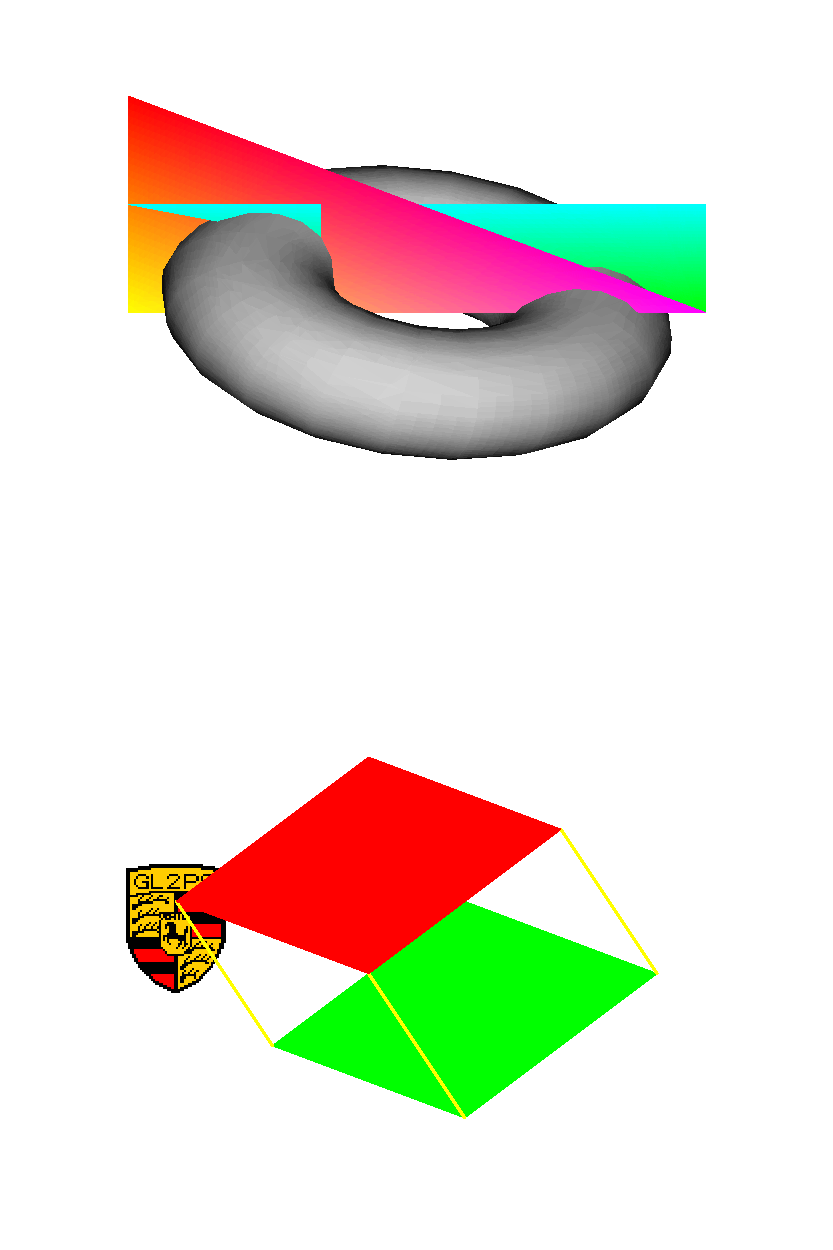
\includegraphics{outLatex}
\end{picture}%
\begin{picture}(400,600)(0,0)
\put(26.9229,389.769){\makebox(0,0)[lb]{Press:}}
\put(26.9229,376.269){\makebox(0,0)[lb]{  s: to save the images}}
\put(26.9229,362.769){\makebox(0,0)[lb]{  t: to alternate between teapot and torus}}
\put(26.9229,349.269){\makebox(0,0)[lb]{  v: to alternate between single and multiple viewport modes}}
\put(26.9229,335.769){\makebox(0,0)[lb]{  q: to quit}}
\put(26.9229,322.269){\makebox(0,0)[lb]{Click and move the mouse to rotate the objects}}
\end{picture}
}
%\caption{Sample output of the test program}
%\end{figure}

\section{Limitations}
\label{sec:limitations}

GL2PS works by capturing the contents of the OpenGL feedback
buffer\footnote{See the description of \dd{glFeedbackBuffer} and
\dd{glRenderMode(GL_FEEDBACK)} in the OpenGL documentation.}. As such, all
the OpenGL operations applied in the pipeline after the creation of the
feedback buffer will be ignored or have to be duplicated by GL2PS (e.g.\
font/image rendering, polygon offset or line stippling---see
sections~\ref{sec:gl2psText}, \ref{sec:gl2psDrawPixels},
\ref{sec:gl2psEnable} and \ref{sec:gl2psPointSize}).

Other limitations include:
\begin{itemize}
\item 
Rendering large and/or complicated scenes is slow and/or can lead to large
output files. This is normal: vector-based images are not destined to
replace bitmap images. They just offer an alternative when high quality
(especially for 2D and small 3D plots) and ease of manipulation (how do you
change the scale, the labels or the colors in a bitmap picture long after
the picture was produced, and without altering its quality?) are important.
\item
Transparency is not supported yet. See the \dd{TODO} file for an explanation
why this may or may not actually be possible.
\item
GL2PS does not support textures, fog effects, etc.
\end{itemize}

% Other implementation Notes:
%
% OpenGL feedback buffer
% describe Simple depth sort
%          3D BSP tree
%          2D BSP image tree for occlusion culling
% float vs. double
% polygon offsets
% PostScript shading
%
% From the GLpr FAQ:
%
% 3. Can GLpr handle 2D texture mapping?
% 
%    Only for pixel-based output (i.e. captured with glpImage()).  GLpr
%    cannot duplicate the effects of texture mapping for vector
%    (move-draw) output.  Unfortunately, the information required is not
%    present in the OpenGL feedback buffer.  
%
% 4. Can GLpr handle 1D texture mapping?
%
%    Not in the present release.  However, future releases may provide
%    support for 1D texture maps (e.g. color lookup).


% \section{Output file formats}
% \label{sec:formats}
%
% GL2PS currently only outputs PostScript (PS) and Encapsulated PostScript
% (EPS) files, as well as \LaTeX\ files for the text fragments. Adding new
% vector output formats should be easy (see the comments in the source code),
% but hasn't been done yet. Amongst the formats we would be interested in
% adding, SVG (http://www.svg.org) is first in line. Meanwhile, you can use
% the excellent pstoedit (http://www.pstoedit.net/) to transform the
% postscript files generated by GL2PS into many other vector formats such as
% xfig, cgm, wmf, etc.

\section{Contributors}
\label{sec:contrib}

\email{Michael Sweet}{mike@easysw.com} for the original implementation of
the feedback buffer parser; 
%
\email{Bruce Naylor}{naylor@comp-graphics.com} for BSP tree and occlusion
culling hints;
%
\email{Marc Um{\'e}}{marc.ume@digitalgraphics.be} for the original list
code;
%
\email{Jean-Fran\c{c}ois Remacle}{remacle@scorec.rpi.edu} for plane equation
fixes; 
%
\email{Bart Kaptein}{B.L.Kaptein@lumc.nl} for memory leak fixes;
%
\email{Quy Nguyen-Dai}{quy@vnilux.com} for output file size optimization;
%
\email{Sam Buss}{sbuss@ucsd.edu} for the \dd{shfill}-based smooth shaded
triangle code;
%
\email{Shane Hill}{Shane.Hill@dsto.defence.gov.au} for the landscape option
implementation;
%
\email{Romain Boman}{r_boman@yahoo.fr} for the Windows dll generation;
%
\email{Diego Santa Cruz}{Diego.SantaCruz@epfl.ch} for the new optimized
shaded triangle code and the \dd{shfill} management;
%
\email{Shahzad Muzaffar}{Shahzad.Muzaffar@cern.ch} and \email{Lassi
Tuura}{lassi.tuura@cern.ch} for the new occlusion culling code and the
improvement of \dd{GL2PS_BEST_ROOT};
%
\email{Guy Barrand}{barrand@lal.in2p3.fr} for his work on
\dd{gl2psDrawPixels} and the new viewport management;
%
\email{Rouben Rostamian}{rostamian@umbc.edu} and \email{Prabhu
Ramachandran}{prabhu@aero.iitm.ernet.in} for various bug reports and fixes.
\section{Links}
\label{sec:links}

Projects similar to \dd{GL2PS} include: Mark J. Kilgard's rendereps
(\url{http://www.opengl.org/developers/code/mjktips/Feedback.html}); Michael
Sweet's GLP library (\url{http://www.easysw.com/~mike/opengl/index.html});
the GLpr library from CEI international (\url{http://www.ceintl.com/}; this
product does not seem to be available anymore).

\email{Toby White}{tow@sdf.lonestar.org} maintains a Python wrapper for
\dd{GL2PS}, available at \url{http://tow.freeshell.org/software.html}.

\section{Versions}

\begin{description}
\item[0.1] (Feb 12, 2000) First distributed version.
\item[0.2] (Feb 20, 2000) Added \dd{GL2PS_POLYGON_BOUNDARY} and
\dd{GL2PS_BEST_ROOT}. API change: changed arguments of \dd{gl2psBeginPage}
and \dd{gl2psText}. Corrected some memory allocation stuff. First version of
this user's guide.
\item[0.21] (Mar 16, 2000) Initialization fixes.
\item[0.3] (Jul 29, 2000) Code cleanup. Added \dd{GL2PS_LINE_STIPPLE}.
\item[0.31] (Aug 14, 2000) Better handling of erroneous primitives.
\item[0.32] (May 23, 2001) Fixed memory leaks.
\item[0.4] (Jun 12, 2001) Added \dd{gl2psPointSize} and
\dd{gl2psLineWidth}. Some code cleanup to allow easier generation of vector
file formats other than postscript.
\item[0.41] (Aug 6, 2001) Fixed string allocation (1 char too
short). Set smaller default line width.
\item[0.42] (Oct 8, 2001) Optimization of output file size. PostScript
header cleanup. Better line width computation.
\item[0.5] (Nov 19, 2001) API change: new \dd{format} and \dd{filename}
arguments for \dd{gl2psBeginPage}. Better PostScript handling of smooth
shaded primitives. Fix handling of zero-length strings. New options for
\LaTeX\ output. Changed (again) the line width computation.
\item[0.51] (Jan 22, 2002) Fixed erroneous drawing of text primitives lying
outside the viewport.
\item[0.52] (Feb 14, 2002) New \dd{GL2PS_LANDSCAPE} option.
\item[0.53] (Mar 11, 2002) New \dd{GL2PSDLL} compilation flag to allow the
generation of a Windows dll.
\item[0.6] (Jun 4, 2002) Fixed some incoherences in string allocation; fixed
sorting of text objects; removed (non functional) occlusion culling code;
fixed handling of color and line width attributes when gl2ps was called
multiple times inside the same program.
\item[0.61] (Jun 21, 2002) Fixed the fix for the sorting of text objects;
introduced tolerance for floating point comparisons.
\item[0.62] (Sep 6, 2002) New \dd{GL2PS_EPS} option to produce Encapsulated
PostScript files; optimized drawing of shaded primitives; new
\dd{GL2PS_NO_PS3_SHADING} option and \dd{gl2psNumShadeColors} function to
control the use of the PostScript level 3 \dd{shfill} operator (usually not
well handled when converting to PDF).
\item[0.63] (Nov 12, 2002) Changed \dd{GLvoid} to \dd{void} to accommodate
some SUN compilers; made subdivision parameters modifiable a posteriori in
the output file; revised documentation.
\item[0.7] (Dec 11, 2002) Occlusion culling (\dd{GL2PS_OCCLUSION_CULL}) is
(finally!) working thanks to the great work of Shahzad Muzaffar; enhanced
\dd{GL2PS_BEST_ROOT}.
\item[0.71] (Dec 13, 2002) Removed C++ style comments inadvertently left in
the code; added example program \dd{gl2psTest.c} to the distribution.
\item[0.72] (Jan 21, 2003) Fixed crash in occlusion culling code; enhanced
documentation.
\item[0.73] (Jan 30, 2003) Minor code cleanup.
\item[0.8] (Mar 10, 2003) API change: \dd{gl2psNumShadeColors} has been
removed and the color subdivision parameters \dd{nr}, \dd{ng} and \dd{nb}
are now given as arguments to \dd{gl2psBeginPage}; API change:
\dd{gl2psBeginPage} takes an additional argument (\dd{viewport}) to specify
the print viewport; new \dd{gl2psDrawPixels} interface to produce mixed mode
PostScript/bitmap output; new \dd{gl2psBeginViewport} and
\dd{gl2psEndViewport} interface to handle multiple OpenGL viewports; fixed
small bug in occlusion culling code; better error handling.
\item[0.81] (Mar 22, 2003) Fixed small typos in comments and documentation.
\item[0.9.0] (Jun 2, 2003) Fixed smooth shading detection for mixed
smooth/flat shaded scenes; new library numbering scheme
(``major.minor.patch'').
\item[0.9.1] (Jun 12, 2003) Fixed two \dd{GL2PS_TEX} output bugs
(\dd{glRenderMode} not reset to \dd{GL_RENDER} + crash when printing empty
scenes); changed default pixmap depth to 8 bits per color component; changed
default line cap to ``Butt cap'' and default line join to ``Miter join''.
\item[0.9.2] (Jul 3, 2003) Improved occlusion culling; new
\dd{GL2PS_USE_CURRENT_VIEWPORT} option.
\end{description}

\end{document}
